% !TEX encoding = UTF-8 Unicode 
% !TEX root = praca.tex

\chapter{Projektowanie i implementacja rozwiązania}

W ramach pracy dyplomowej opracowano aplikację \texttt{gptester}, , której celem jest statyczna analiza kodu w poszukiwaniu podatności bezpiec
zeństwa oraz proponowanie ich napraw. Aplikacja wykorzystuje modele GPT-4, lub GPT-3.5 dostarczane przez OpenAI i jest zaprojektowana do działania z linii komend, z wynikami zapisywanymi w pliku markdown.

\section{Opis rozwiązania}

Program \texttt{gptester}
jest narzędziem do statycznej analizy kodu, które korzysta z modelu GPT-4 do generowania raportów dotyczących jakości kodu i proponowania napraw. Głównym celem programu jest bezpieczeństwo kodu, które ma być w przyszłości rozszerzone. Aplikacja została napisana w języku Python, a model GPT-4 jest dostarczany przez OpenAI. Program jest przeznaczony do uruchamiania z linii poleceń, a wyniki są zapisywane w pliku markdown. Program można uruchomić z następującymi argumentami:

\begin{verbatim}

    ./main.py -h
    usage: main.py [-h] [--model MODEL] [--input INPUT] [--output OUTPUT]
\end{verbatim}

\begin{figure}
    \centering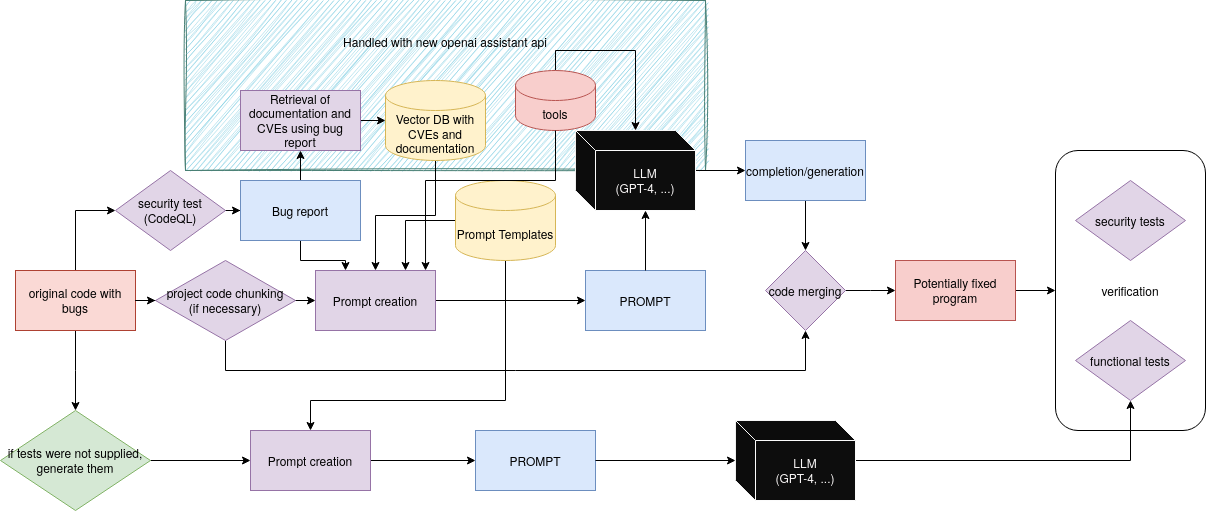
\includegraphics[width=.6\textwidth]{img/gptester.drawio.png}
    \caption{Schemat blokowy działania aplikacji}  \label{rys:schemat}
    \end{figure}
    
    Na rysunku \ref{rys:schemat} \dots